\Chapter{Processz ütemezés}

\Section{Az ütemezési probléma}

\Section{Elterjedt ütemezési stratégiák}

\SubSection{$\mathcal{O}(n)$}
Az $O(n)$ ütemező, amelyet a Linux kernelben használtak 2.4 és 2.6 verziók között. A müködési elve egyszerűnek mondható, mivel végigiterál az összes futtatható processzen, kiszámolja a prioritásaikat, majd a "legjobbat" választja meg futásra. A "legjobb" jelző, a processzekhez rendelt nice értékből és a felhasználatlan időszeletből kalkulálódik.
Ez egy $O(n)$ műveletigényű algoritmus volt, ahol az $n$ a futtatható processzek számát jelölte. Emiatt nagy processzámnál nem volt elég effektív és a valós idejű processzek így kiszámíthatlanok lettek.
\SubSection{$\mathcal{O}(1)$}
Az $O(1)$ ütemezőt Linux kernel 2.6-os verziótól 2.6.22 ig használták. Konstans idő alatt választott következő processzt futásra, emiatt nagy processz szám mellett is használható volt, az $O(n)$-es ütemezővel ellentétben.
A processzeket két részre osztja, típus szerint. A valós idejű processzek 0-99-ig kaptak prioritás szinteket, amíg a normál processzek(Batch vagy inveractive) 100-139-ig. Itt a 100-as prioritás jelöli a legfontosabb processzt, amíg a 139 a legkevésbé fontosat. Normál processzekhez egy alapértelmezett 120-as statikus prioritást rendeltek. A nice paranccsal tudjuk ezt az alapértelmezett prioritást változtatni.
\begin{cpp}
\$nice -n N ./a.out 
\end{cpp}
Ahol az N értéke +19 és -20 között mozoghat.

Normál processzek ütemezésénél, processzoronként, két listát tart nyilván amiben tárolódnak a futásra kész processzek. (Active run queue, Expired run queue)
Mindig az aktív listából választja a legfontosabb processzt, futásra. Amikor végzett, a futó processz átkerül az expired run queue-ba, egy új dinamikusan számolt prioritással.
Emiatt ahogy haladunk előre az időben az active run queue-ból folyamatosan fogynak el a processzek.  Amikor az active run queue végzett a processzekkel, a két lista felcserélődik és folyatatódik a végrehajtás az új listával.
Annak érdekében hogy meglehessen különböztetni a batch és az interactive processzeket, egy úgynevezett "bonus" valtozot tartunk nyilván, ami dinamikus prioritás számításnál fog előkerülni. Ennek az értéke 0 és 10 között mozoghat.
\begin{cpp}
dynamic priority = MAX(100, MIN(static priority - bonus + 5), 139)) 
\end{cpp}
Amikor a bonus változó értéke kisebb mint 5, arra utal hogy kevesebb interakciót fog végezni a felhasználóval, így több cpu lázas szakasza lesz a processznek élete során. Konvergálódik a 139-es prioritás felé, ezt a processz típust nevezzük batch processznek.(Kevésbé lesz fontos) 
Ha a bonus változó értéke több mint 5 lesz, valószínűleg a processz élete során sok interakcióra lesz szüksége a felhasználóval, tehát ez egy interactive processz (másnéven I/O lázas). A prioritása konvergálódik a 100 felé. Az interactive processzek általában nem fejezik be az időszeletüket amit kapnak, ezért nekik nagyobb időszeletet kell hogy adjunk. Így bizonyosodhatunk meg arról hogy ténylegesen be tudja fejezni az instrukció sorozatot, és majd ha kész, lemond önszántából a CPU-ról.

Az időszelet meghatározása úgy történik, hogy amelyik processz kevesebb mint 120-as prioritással rendelkezik, nagyobb időszeletet kap, 120-nál nagyobb prioritású processzek pedig kevesebbet.
\begin{cpp}
if priority < 120 
	time slice = (140 - priority) * 20    milliseconds 
else
	time slice = (140 - priority) * 5   milliseconds 
\end{cpp}

\begin{figure}[h]
\centering
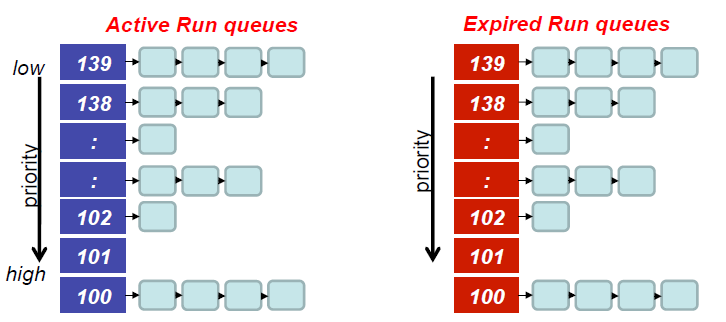
\includegraphics[width=\textwidth]{images/activeexpiredrunqueue.png}
\caption{Active and Expired Run queues}
\label{fig:Active and expired runqueues}
\end{figure}

\SubSection{Completely Fair Scheduler}
A "Completely Fair Scheduler", azaz (CFS) ütemezőt még Molnár Ingo mutatta be 2007 júliusában, amit Linus Torvalds be is olvasztott a Linux kernel(2.6.23) rendszermagjába. A korábbi $\mathcal{O}(1)$ ütemező komponenseit, mint például: az aktív és lejárt folyamatok tömbje, interaktív processzek azonosítása, prioritás alapú időszelet koncepció, eltávolították, a hatékonyság javíásának érdekében. 

Az alapvető adatstruktúra az ütemezőben a folyamatok Run-queue. A run-queue-t a \textit{kernel/sched.h}-ben definiálták, mint \textit{struct rq}. Maga a run-queue egy lista ami a futtatható entitásokat tartalmazza, minden processzorhoz tartozik egy run-queue. A run-queue-nak, különböző területei vannak mint például cfs, real time, deadline run queue-k.
Mindegyiknek megvan a saját ütemezője.
\begin{cpp}
struct rq {
      struct cfs_rq cfs;  // completely fair scheduler
      struct rt_rq rt;    // real-time scheduler
      struct dl_rq dl;    // deadline scheduler
}
\end{cpp}

%\begin{figure}[h!]
%\centering
%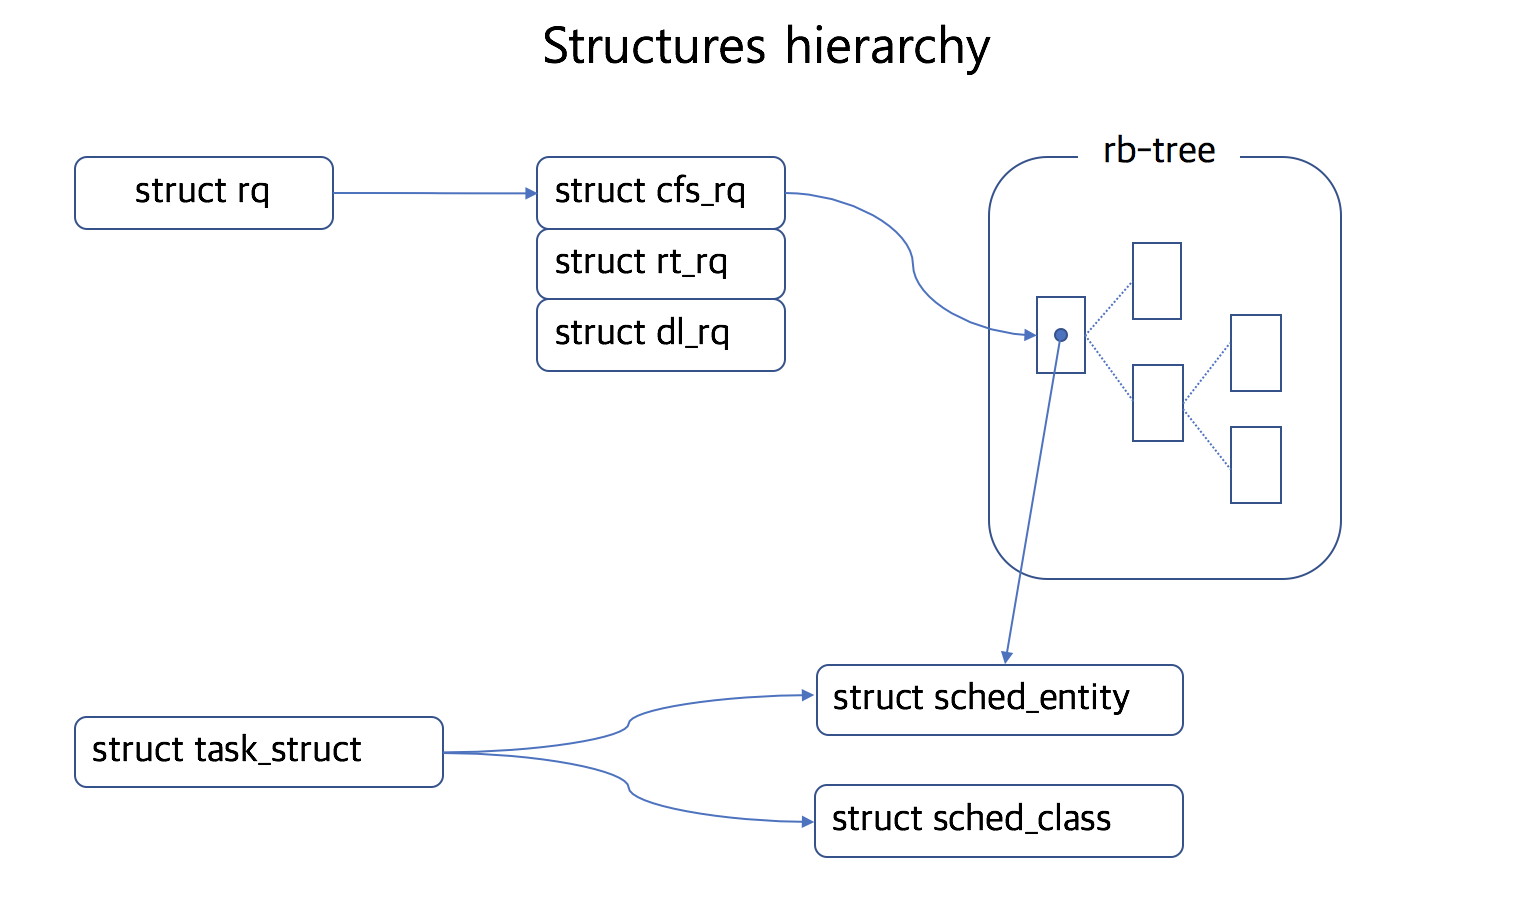
\includegraphics[width=\textwidth]{images/structures.png}
%\caption{Struktúra hierarchia}
%\label{fig:structurehierarchi}
%\end{figure}
Az ideális ütemezés érdekében, a CFS algoritmus felosztja a processzor időszeletet a processzek között és minden processz $(100/N)\%$ részt kap meg, ahol az $N$ a processzek számát jelöli.
\begin{table}[h]
\centering
\caption{A processz végrehajtásához szükséges idő}
\label{tab:processtimes}
\begin{tabular}{|c|c|}
\hline
Processz & idő \\
\hline
A & 8ms \\
B & 4ms \\
C & 16ms \\
D & 4ms \\
\hline
\end{tabular}
\end{table}

\begin{table}[h]
\centering
\caption{A processzekre jutó időszeletek}
\label{tab:timeslices}
\begin{tabular}{|c|c|c|c|c|c|c|c|c|}
\hline
A & 1 & 2 & 3 & 4 & 6 & 8 & & \\
B & 1 & 2 & 3 & 4 & & & & \\
C & 1 & 2 & 3 & 4 & 6 & 8 & 12 & 16 \\
D & 1 & 2 & 3 & 4 & & & & \\
\hline
\end{tabular}
\end{table}

Minden futásra képes processzhez tartozik egy virtuális futásidő (vruntime). Amint egy processzt megválasztunk $t$ miliszekundum futásra, ezt a $t$-t hozzáadjuk a virtuális futásidejéhez a processznek.(vruntime$+=t$). Emiatt a virtuális futásidő monoton növekvő lesz.
Amikor az óra eszköztől érkezik egy megszakitás, az ütemező mindig a legkisebb virtuális futásidővel rendelkező processzt választja futásra. Kontextusváltás történik, amint az aktuálisan futó processznél, lesz kisebb virtuális futásidővel rendelkező processz. Emiatt időszeletek mérete dinamikus. 
A CFS ütemező a következő időszeletre történő task választásához, egy piros-fekete fát használ. A fában a csomópontok egy-egy futásra képes taszkot reprezentál. A taszkok elhelyezkedése a fában a virtuális futásidejükhöz mérten történik. A fa bal oldalában mindig kevesebb vruntime-mal rendelkeznek a taszkok mint a jobb oldalán. A balszélső csomópontban mindig az a taszk helyezkedik el amelyik a legkevesebb a vruntime-mal rendelkezik.(Erre egy min\_vruntime változót tartunk nyilván). Az önszabályzó képessége miatt alkalmaznak piros-fekete fát. Emellett minden művelet futási ideje $O(log\ n)$ és a fába történő beszúrás/törlés is gyorsan végezhető.
A prioritás kezelés, virtuális futásidőhöz történő súlyok hozzárendelésével történit, így amikor egy processz $t$ miliszekundumig fut:
$$vruntime+=t*(weight\ based\ on\ nice\ of\ process)$$
Minél alacsonyabb a prioritás száma egy processznek, annál fontosabb végrehajtás szempontjából.
\begin{figure}[h]
\centering
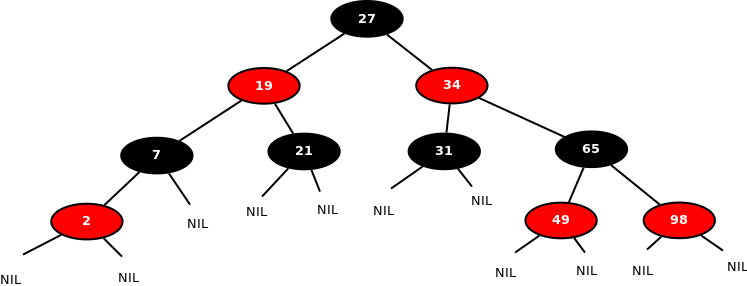
\includegraphics[width=\textwidth]{images/rb_tree.png}
\caption{Piros fekete fa a processz prioritás értékekkel}
\label{fig:rb_tree}
\end{figure}
